\documentclass{beamer}
\usepackage[serbian]{babel}
\usetheme{Boadilla}
\usecolortheme{seahorse}
\usefonttheme{serif}

\usepackage{lipsum}
\usepackage{graphicx,xcolor}
\usepackage{amsmath,amssymb,amsfonts}

%\AtBeginSection[]{ 
    %\begin{frame}{Outline} 
   %     \tableofcontents[currentsection] 
 %   \end{frame} }

\title{Robotika u 2022.}
\subtitle{}
\institute[Tehničko i naučno pisanje]{Matematički fakultet\\Univerziteta u Beogradu}
\author[]{Đuro Cerović\\Marko Cvijetinović\\Luka Matić\\Mihajlo Radojević}
\date{12/2022}
%\titlegraphic{
\includegraphics[width=2cm]{images/logo/iiserm_logo.jpg}}

\begin{document}

\begin{frame}
\titlepage
\end{frame}


\section{Uvod}
%\input{segments/1_intro}
\begin{frame}{Uvod}
    \begin{itemize}
        \item Uticaj ubrzanog razvoja nauke i tehnike na industriju i društvo
        \item Ulaganje u razvoj novih tehnologija  od kojih je jedna robotika
        \item Robotika je nova nauka koja obuhvata više naučnih polja
        \item Robot kao zamena za ljudski napor
        \item Asimovljevi zakoni robotike
    \end{itemize}
    \begin{figure}
        \centering
        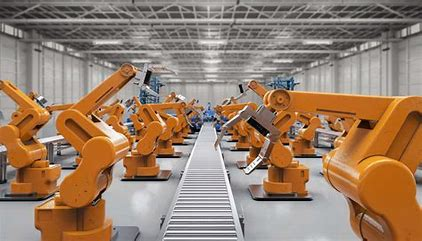
\includegraphics[scale=0.45]{roboti.png}   
    \end{figure}
\end{frame}
 
\section{Saradnički roboti}
\begin{frame}{Saradnički roboti}
    \begin{itemize}
        \item Rast potražnje zbog pandemije
        \item Preuzimaju suvoparne, prljave i opasne poslove
        \item Automatizacija procesa dovodi do veće preciznosti i efikasnosti 
        \item Imaju veliku primenu u fabrikama 
    \end{itemize}
    \begin{figure}
        \centering
        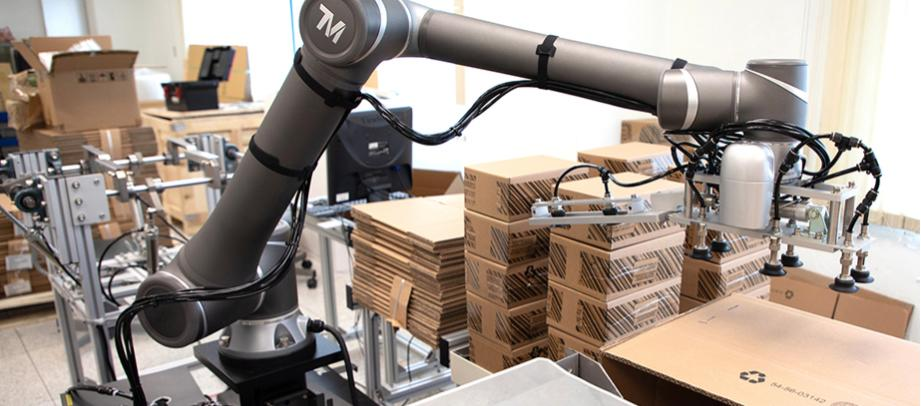
\includegraphics[scale=0.25]{Cobot.jpg}
    \end{figure}
\end{frame}

\section{Roboti dostavljači}
\begin{frame}{Roboti dostavljači}
    \begin{itemize}
        \item Nastali radi smanjenja kontakta izmedju ljudi
        \item Fleksibilniji od ljudi jer mogu da rade 24/7
        \item Povećanje potražnje za brzom dostavom doprinosi njihovoj popularnosti
    \end{itemize}
    \begin{figure}
        \centering
        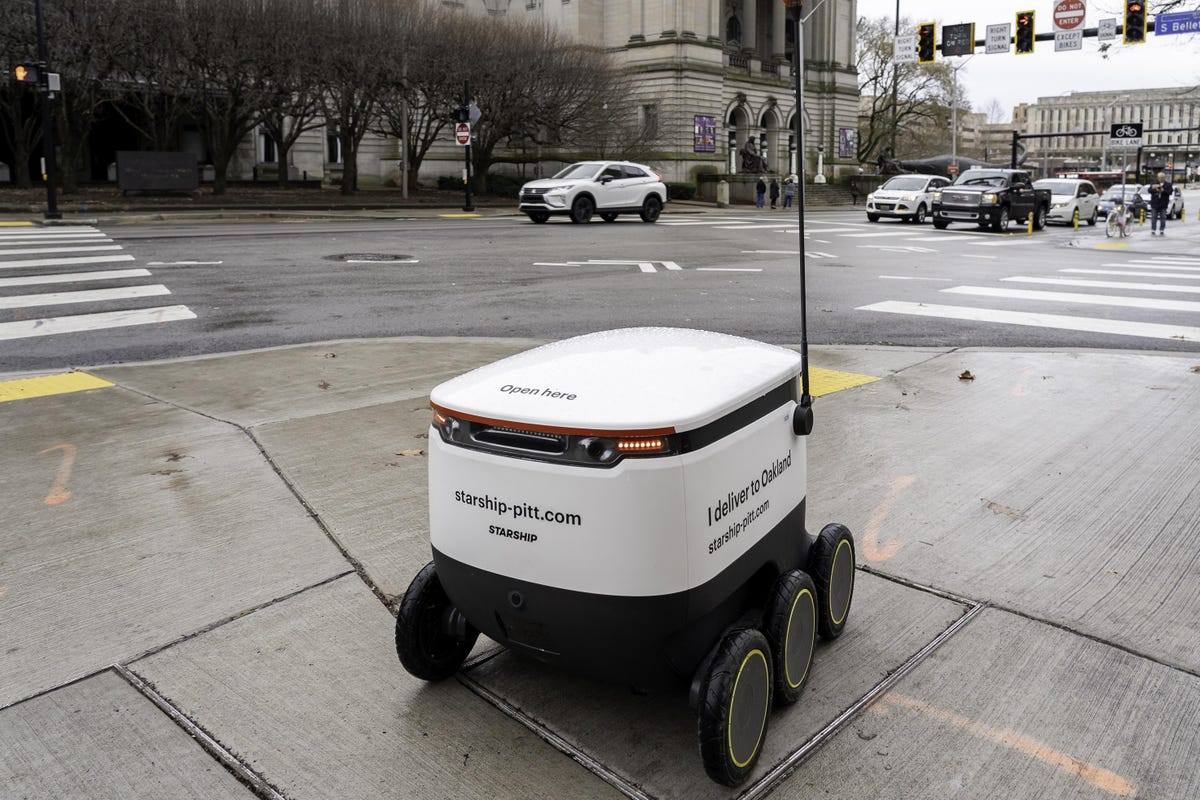
\includegraphics[scale=0.15]{DeliveryRobot.jpg}
    \end{figure}
\end{frame}

\section{Prediktivno održavanje}
\begin{frame}{Prediktivno održavanje}
    \begin{itemize}
        \item Robotika može da uštedi ogromne količine novca, ali takođe dolazi sa troškovima održavanja.    
        \item Koristi se tehnologija kao što je senzor Interneta koja prati perfomanse i fizičko stanje robota
        \item IoT i tehnologije daljinskog otkrivanja i praćenja postaju posebno popularne u skladištima, gde se roboti koriste za sve.
    \end{itemize}
    \begin{figure}
        \centering
        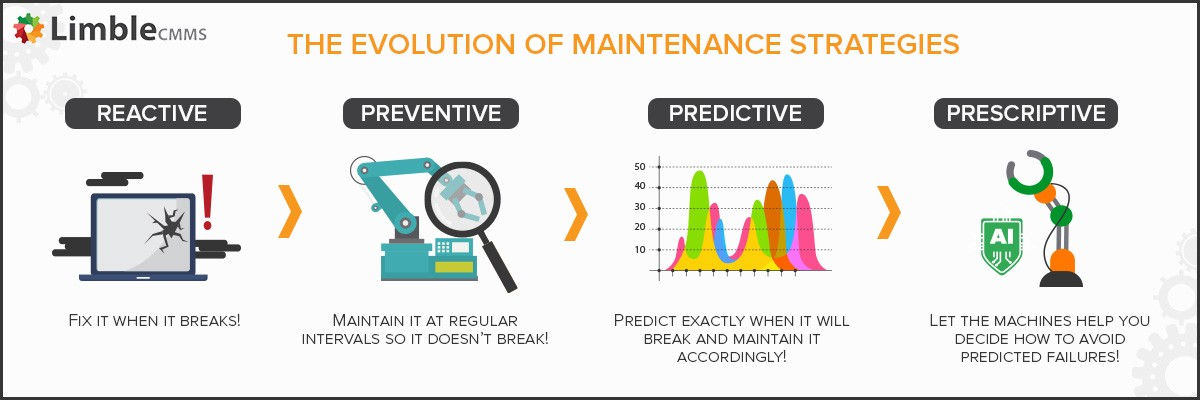
\includegraphics[scale=0.20]{dijagram.jpeg}
    \end{figure}
\end{frame}

\section{Povećanje kompatibilnosti}
\begin{frame}{Povećanje kompatibilnosti}
    \begin{itemize}
        \item Sa toliko inovacija u robotici, raznovrsnost i prilagođavanje postaju briga za neka preduzeća.    
        \item U 2022. sve više programera robotike ima to na umu.
        \item Ovaj trend obuhvata veštačku inteligenciju i mašinsko učenje, ali i druge robote.
        \item Tržišna prednsost za robote je da budu lako kompatibilni sa drugim,   potpuno drugačijim robotima.
    \end{itemize}
    
\end{frame}
\section{Kuhinjski roboti}
\begin{frame}{Kuhinjski roboti}
   \begin{itemize}
      \item Primena robotike u kuhinjskim poslovima
      \item Primeri robotike u prehrambenoj industriji
      \item Funkcionisanje Robota za pravljenje pice
      \item Doprinos robotike u kuhinjskim poslovima
       \end{itemize}

   
   \begin{figure}
       \centering
       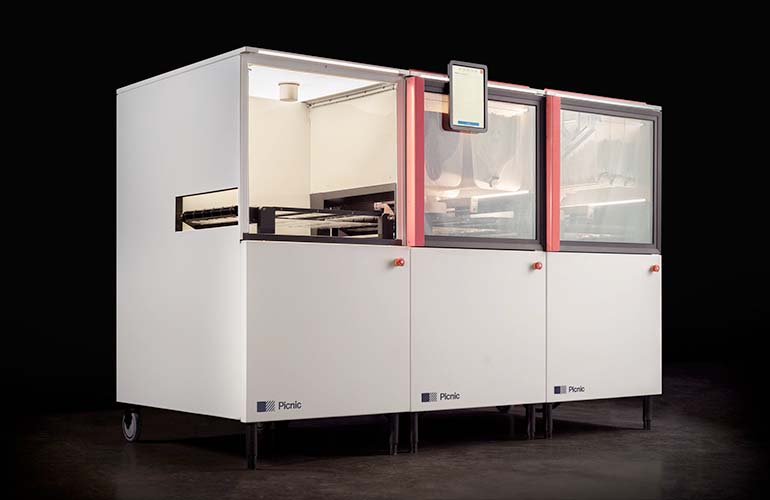
\includegraphics[scale=0.20]{picnic-featured-image-web.jpg}
   \end{figure}
\end{frame}  
\section{Primena veštačke inteligencije u robotici}
\begin{frame}{Primena veštačke inteligencije u robotici}
   \begin{itemize}
       \item Razvoj veštačke inteligencije u robotici
       \item Njena primena
       \item Benefiti koje je donela veštačka inteligencija
   \end{itemize}
    
\end{frame}
    


\section{Conclusion}
%\input{segments/4_conclude}


%\section*{References}
%\begin{frame}
  %  \frametitle{References}
  % \bibliographystyle{amsalpha}
  %  \bibliography{ref.bib}
%\end{frame}

\end{document}
